\chapter{Einführung in modulare Assets}
In diesem Kapitel werden grundlegende Aspekte der Modularität erläutert.
\section{Begriffserklärung und Definition}
Folgende Begriffe sind für die Thesis relevant und werden deshalb in diesem Abschnitt definiert und erläutert:
\begin{itemize}
\item Modularität
\item Kit
\item Asset
\item Game-Engine
\end{itemize}
\subsection{Modularität}
Wikipedia definiert Modularität wie folgt:
\begin{quote}
\enquote{Modularität (auch Baustein- oder Baukastenprinzip) ist die Aufteilung eines Ganzen in Teile, die als Module (...) oder Bausteine bezeichnet werden. Bei geeigneter Form und Funktion können sie zusammengefügt werden oder über entsprechende Schnittstellen interagieren. Bei einem modularisierten Aufbau werden Systeme aus Bauteilen entlang definierter Stellen (...) zusammengesetzt.
} \parencite{moduwiki}
\end{quote}
Bei der Entwicklung von Videospielen kommt Modularität beispielsweise zum Einsatz, um aus kleinen, wiederverwendbaren Einzelteilen verschiedene Permutationen größerer Gebilde zu erzeugen \parencite{Meler}. Diese Elemente können, wie im obigen Zitat beschrieben, an definierten Stellen mit einander verbunden werden.
\par
Die Verwendung sogenannter \enquote{Kits} erlaubt die Integration von Modularität in die Spieleentwicklung \parencite{Burgess}.
\newpage
\subsection{Kit}
Ein \enquote{Kit} (engl., Bausatz) ist eine Sammlung aus Elementen, die nach einem definierten System miteinander verbunden werden können. Ein Kit kann beispielsweise aus mehreren Elementen eines Rohrs bestehen, durch dessen Kombination verschiedene, größere und komplexere Systeme gebaut werden können (vgl. Abbildung \ref{pipes}). \parencite{Burgess}
\begin{figure}[H]
\centering
  \makebox[\textwidth]{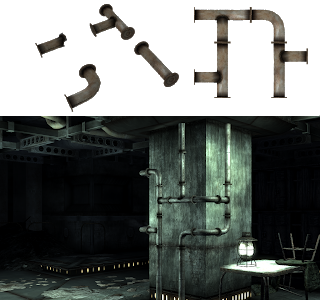
\includegraphics[width=\linewidth]{bilder/pipes}}
  \caption{Beispielhaftes modulares Kit eines Rohr-Systems aus \textit{Fallout 3} (Bethesda Softworks, 2008), \parencite{Burgess}.}
\label{pipes}
\end{figure}
\subsection{Asset}
Die Elemente die ein Kit ausmachen werden \enquote{Assets} genannt und von G. Rehfeld folgendermaßen definiert:
\begin{quote}
\enquote{Assets sind die benötigten Bestandteile eines Spiels. Bei einem Analogspiel die unterschiedlich farbigen Pöppel und Karten, das Spielbrett und die  Würfel. In einem Digitalspiel handelt es sich um alle Objekte, die im Spiel auftauchen: Die Modelle und animierten Figuren, die Spieler und Lebewesen der Welt darstellen, feste Objekte der Spielwelt wie Autos, Bäume, Häuser, Gegenstände wie Waffen, Kleidung etc. Also alles, was man im Film als „Prop“ oder „Requisite“ bezeichnet und dazu dient, die Atmosphäre des Spiels so klar wie möglich darzustellen.} \parencite[S.\,53-54]{rehfeld}
\end{quote}
Nach dieser Definition umfasst \enquote{Asset} viele verschiedene Elemente. In dieser Arbeit wird \enquote{Asset} hauptsächlich für die Bezeichnung fester Objekte in der Spielwelt genutzt und umfasst somit beispielsweise Gebäude, Höhlen oder Raumschiffe.
\subsection{Game-Engine}
Für die Entwicklung von Videospielen werden Game-Engines genutzt. Zu den aktuell bekanntesten gehören Unity und Unreal Engine \parencite{BestEngine}.
Jeff Ward, Spieleprogrammierer und Dozent, definiert die Leistung und den Nutzen von Game-Engines wie folgt:
  \begin{quote}
  \enquote{...it exists to abstract the (sometime platform-dependent) details of doing common game-related tasks, like rendering, physics, and input, so that developers (artists, designers, scripters and, yes, even other programmers) can focus on the details that make their games unique.
\par
Engines offer reusable components that can be manipulated to bring a game to life. Loading, displaying, and animating models, collision detection between objects, physics, input, graphical user interfaces, and even portions of a game's artificial intelligence can all be components that make up the engine.} \parencite{Engine}
  \end{quote}
Durch Spiele-Engines wird das Entwickeln von Spielen also erheblich erleichtert \parencite{Engine}. Für eine performantes Spiel und eine fehlerfreie Darstellung müssen tiefgreifende Aspekte der Engine verstanden werden. Daher wird im Folgenden auf die Funktionsweise von Realtime Rendering eingegangen, welches für die Darstellung in Spielen genutzt wird.
\section{Geschichte von Modularität in Videospielen}\label{Geschichte von Modularität }
Ein frühes Beispiel für Modularität in Videospielen ist \textit{Super Mario Bros.} (Nintendo, 1987) für das Nintendo Entertainment System. Die Level des Spiels wurden auf Kästchenpapier entworfen, also auf einem Raster, mit dem die digitalen Koordinaten für das Spiel definiert werden konnten (vgl. Abbildung \ref{marioAnalog}). Nach dem Designprozess wurden die Level von Programmierern Block für Block in das Spiel implementiert \parencite{marioAnalog}.
\begin{figure}[H]
\centering
  \makebox[\textwidth]{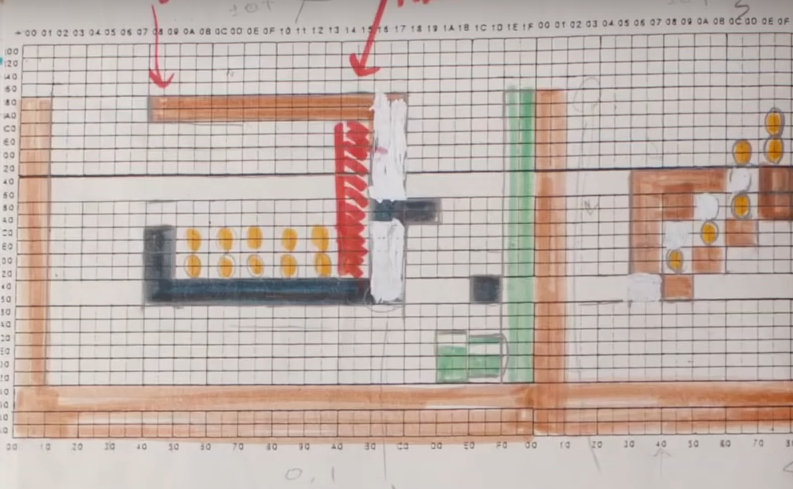
\includegraphics[width=0.68\textwidth]{bilder/marioAnalogAuschschnitt}}
  \caption{Ausschnitt eines Original Entwurfs eines \textit{Super Mario Bros.} Levels. In Anlehnung an \parencite{marioAnalog}.}
\label{marioAnalog}
\end{figure}
\enlargethispage{10.5pt}
\begin{figure}[H]
\centering
  \makebox[\textwidth]{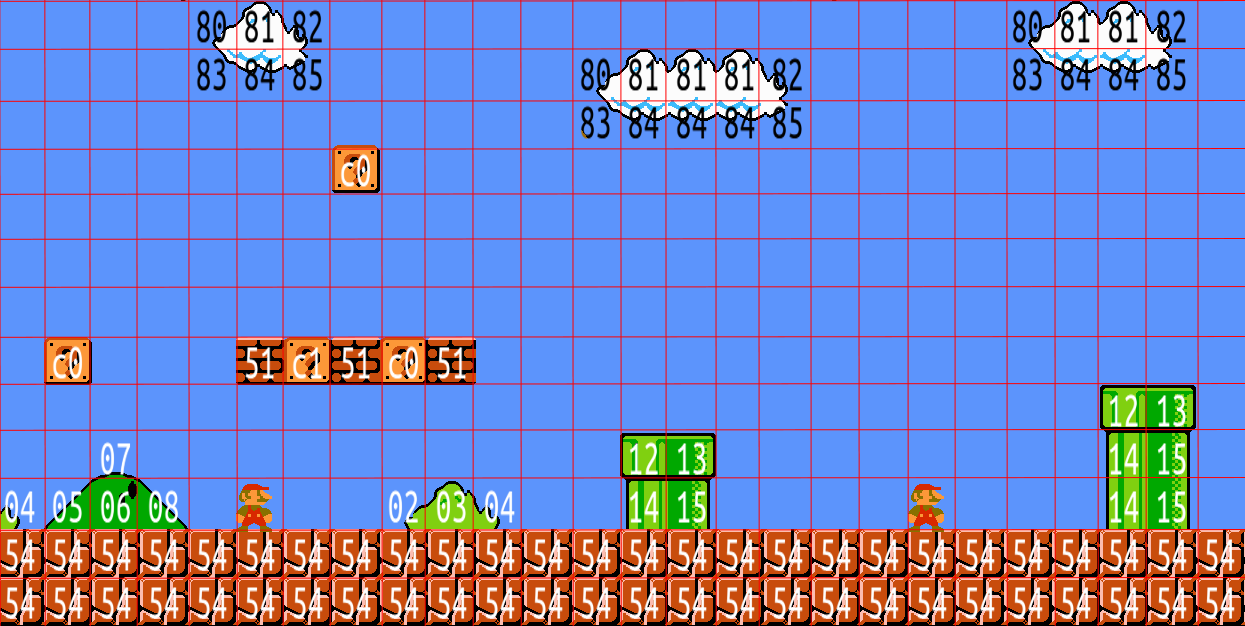
\includegraphics[width=0.68\textwidth]{bilder/SuperMarioBrosAnalysis}}
  \caption{Analyse der Tiles in \textit{Super Mario Bros.}. In Anlehnung an \parencite{MarioTiles}.}
\label{MarioImage}
\end{figure}
\vspace{-10.5pt}
%\begin{figure}[!h]
%\centering
%  \subfloat[][Ausschnitt eines Original Entwurfs eines \textit{Super Mario Bros.} Levels. In Anlehnung an \parencite{marioAnalog}.]{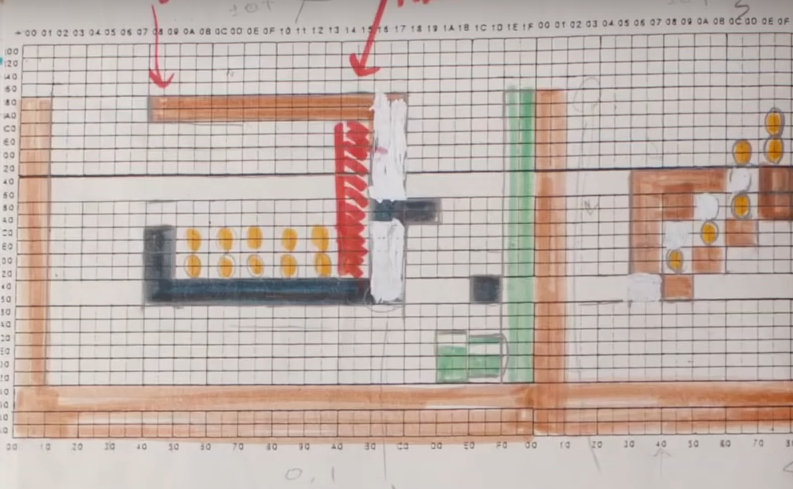
\includegraphics[width=0.42\linewidth]{bilder/marioAnalogAuschschnitt}\label{marioAnalog}}%
%  \qquad
%  \subfloat[][Analyse der Tiles in \textit{Super Mario Bros.}. In Anlehnung an \parencite{MarioTiles}.]{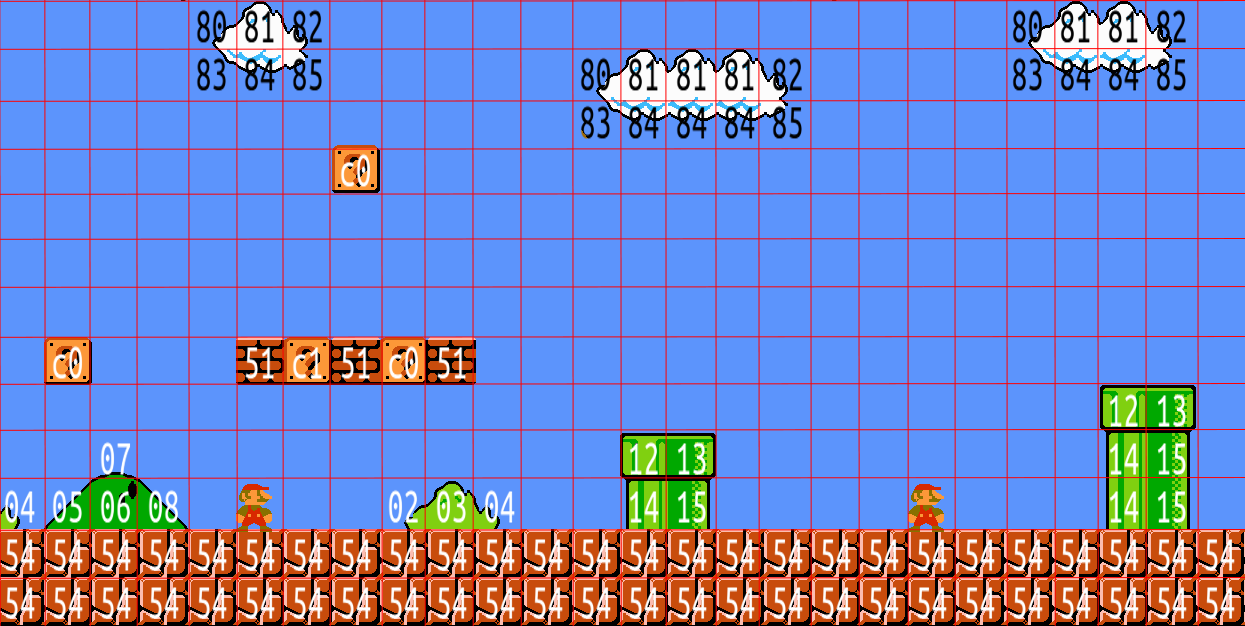
\includegraphics[width=0.52\linewidth]{bilder/SuperMarioBrosAnalysis}\label{MarioImage}}%
%  \caption{Analoges und digitales Level-Layout von Super Mario Bros.}%
%\end{figure}
\par
Alle Elemente der Level wurden mit Hilfe von Tiles\footnote{Ein Tile ist eine Grafik, die mosaikartig zusammengesetzt ein größeres Gesamtbild ergibt.} dargestellt. Wie in der Abbildung \ref{MarioImage} zu sehen, besteht dieser Ausschnitt des Levels aus nur wenigen verschiedenen Tiles. Sie sind in einem Raster angeordnet und wurden so aufgebaut, dass sie nahtlos aneinanderpassen. So ließen sich mit nur wenigen Sprites\footnote{Ein Sprite ist eine zweidimensionale Grafik.} beliebig große Objekte erstellen und ganze Level bauen. Das grüne Rohr kann zum Beispiel mit den Stücken 14 und 15 beliebig verlängert werden. Das gleiche gilt für die Wolken und die Tiles 81 und 84. Diese modulare Herangehensweise erlaubte es den Entwicklern trotz der Hardware-Speicher-Limitierungen von damals größere Level zu entwickeln \parencite{Mario}.
\par
Die fortschreitende Technologie brachte die Möglichkeit mit sich, Spiele im dreidimensionalen Raum zu entwickeln, was als logischen Schluss hatte, dass die meisten Spiele fortan in 3D entwickelt wurden \parencite{GameHistory}. Der Schritt in die dritte Dimension brachte sowohl in der Programmierung als auch beim Design der Spiele neue Hindernisse mit sich, die es zu überwinden galt.
\par
Trotz der fortgeschrittenen Technik waren Speicherplatz und Rechenleistung noch nicht so ausgereift wie heute und stellten ein Problem dar, wenn große Welten entwickelt werden sollten. Spiele wie \textit{The Elder Scrolls II: Daggerfall}\footnote{Daggerfall ist ein Open-World-Action-Rollenspiel welches aus der Egoperspektive gespielt wird.} (Bethesda Softworks, 1996) wussten sich durch den Einsatz der Modularität und Prozeduralität zu helfen und umgingen dieses Problem somit \parencite{Fallout4}. Die geschickte Kombination von Modularität und Prozeduralität erlaubte den Entwicklern mit Hilfe weniger modularer Dungeon-Blöcke eine Vielzahl unterschiedlich wirkender Dungeons zu generieren \parencite{Fallout4}. Die algorithmisch erstellten Level sorgten so für sehr viel mehr Abwechslung, wodurch in nur kurzer Zeit etwa 15.000 Orte generiert werden konnten \parencite{Daggerfall}. Die Welt von \textit{Daggerfall} bestand aus zweidimensionalen Sprites, die in einer dreidimensionalen Umgebung platziert wurden. Obwohl diese Technik sich deutlich von der heutigen unterscheidet, ähneln die Modularitätsansätze in \textit{Daggerfall} dennoch denen aktueller Spiele.
\par
\begin{figure}[!h]
\centering
  \subfloat[][Übersicht eines Dungeons aus \textit{Daggerfall}.]{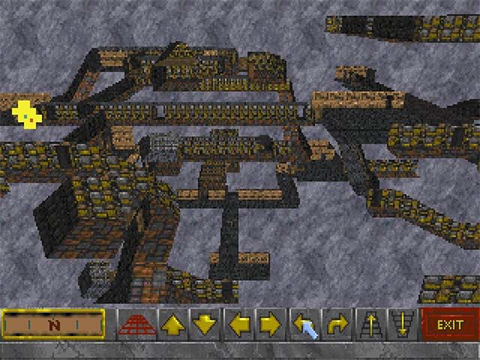
\includegraphics[height=4.4cm]{bilder/Daggerfall}}%
  \qquad
  \subfloat[][Übersicht eines Dungeons aus \textit{Morrowind}.]{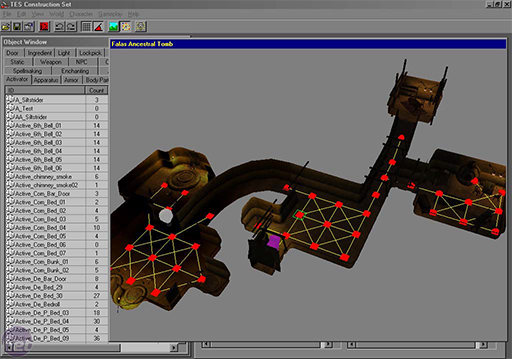
\includegraphics[height=4.4cm]{bilder/Morrowind}}%
  \caption{Beispiele für Modulare Dungeons \parencite{Fallout4P}.}%
\end{figure}
\newpage
\textit{The Elder Scrolls III: Morrowind} (2002) von Bethesda Softworks ist der erste Teil der \textit{Elder Scrolls}-Reihe, der komplett dreidimensionale Assets nutzte und neben der Egoperspektive auch über eine Third-Person-Perspektive verfügte. Auch in diesem Teil wurden die Dungeons mit Hilfe modularer Assets erstellt \parencite{Fallout4}. Dieses Mal wurden sie allerdings nicht prozedural generiert, sondern von Hand erstellt und genau von den Level-Designern geplant. Folglich war die Welt von \textit{Morrowind} kleiner, aber realistischer aufgebaut, als die ihres Vorgängers \parencite{Morrowind}. \textit{Morrowind} hatte nur 0.01\% der Größe seines Vorgängers \parencite{Daggerfall}, was ein Beispiel für Möglichkeiten von Modularität und prozeduraler Generierung ist. Ähnlich zu dem System aus \textit{Super Mario Bros.} (Abschnitt \ref{Geschichte von Modularität }) arbeitet der Level-Editor aus \textit{Morrowind} mit einem Raster, auf dem verschiedene modulare Tiles aneinander gesteckt werden können. Dadurch entstehen aus den einzelnen Modulen komplette Höhlensysteme \parencite{Fallout4}.
\par
Der in \textit{Morrowind} genutzte Ansatz wurde auch bei \textit{The Elder Scrolls IV: Oblivion} (Bethesda Softworks, 2006) angewandt. Für einen abwechslungsreicheren Look wurden modulare Assets auch mit vielen individuellen Assets kombiniert. \parencite{Fallout4}
\par
Für \textit{The Elder Scrolls V: Skyrim} (Bethesda Game Studios, 2012) wurde 
das in \textit{Morrowind} und \textit{Oblivion} genutzte System für Modularität weiter verbessert. Zu Beginn der Entwicklung wurden Kits definiert, die jeweils einen Bereich der Spielwelt abdecken sollten. Die Kits beinhalteten Assets, mit denen natürlichere Formen, wie Höhlen und Tunnel, dargestellt werden konnten. Dadurch war es möglich, sich von dem kastenförmige Erscheinungsbild, welches modulare Ansätze vorher prägte, zu entfernen.
\begin{figure}[H]
\centering
  \makebox[\textwidth]{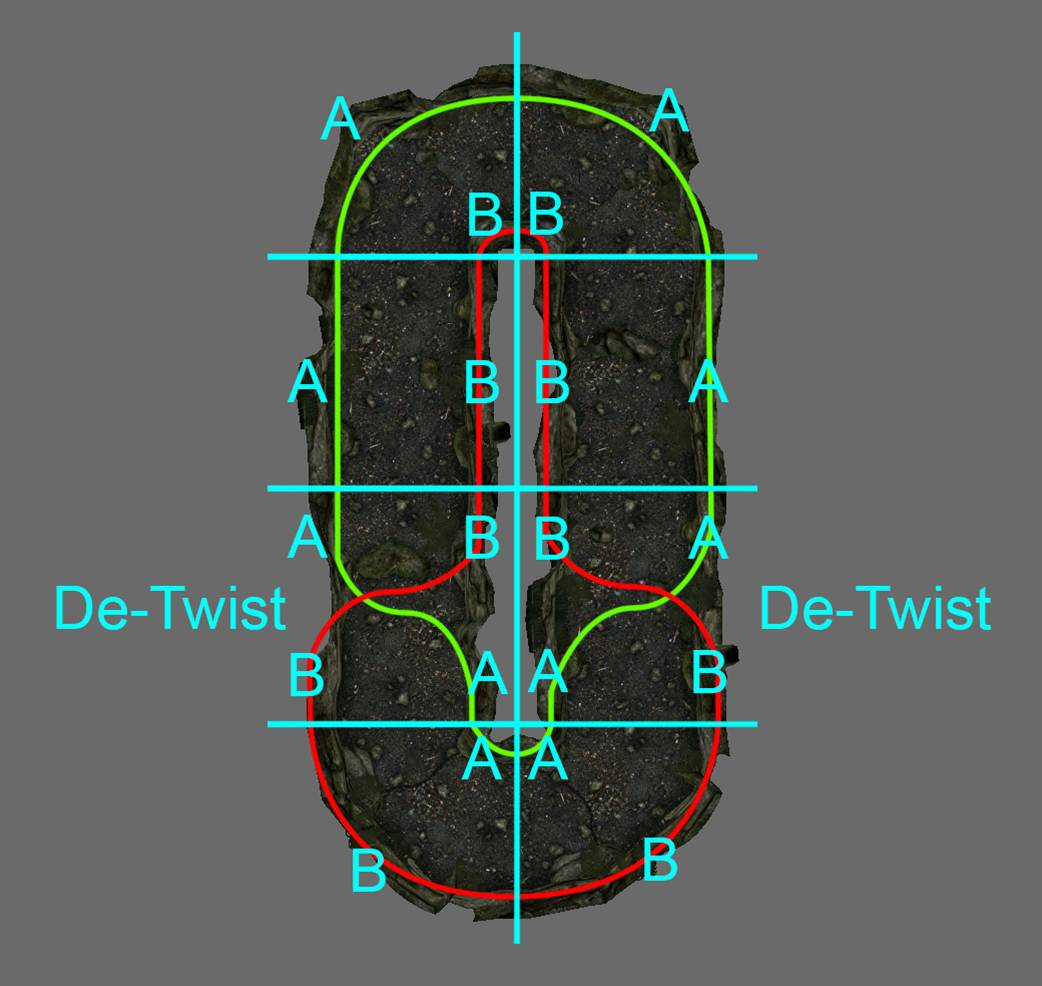
\includegraphics[width=0.6\textwidth]{bilder/asy1}}
  \caption{Asymmetrische Tunnelmodule aus \textit{Skyrim} \parencite{Burgess}.}
\label{ForHonorImage}
\end{figure}
\vspace{-10.5pt}
Hierfür wurden unter anderem asymmetrische Module entwickelt, die sich nur in eine Richtung miteinander verbinden ließen. Die Nutzung asymmetrischer Assets verursacht mehr Arbeit, diese wird aber durch die höhere visuelle Qualität gerechtfertigt. Durch für alle Kits definierte Regeln konnten die Assets der verschiedenen Kits auch gut untereinander kombiniert werden. Dank dieser Technik reichten schon sieben verschiedene Kits, für genügend Abwechslung in den über 400 Leveln \textit{Skyrims}. Bethesdas Hauptziel beim Einsatz der Modularität war, trotz weniger Mitarbeiter möglichst viele Inhalte generieren zu können. Von den zur Zeit der Entwicklung 90 Mitarbeitern im Entwicklungsteam waren nur zehn für die Level-Erstellung zuständig. \parencite{Burgess}
\par
Mittlerweile ist Modularität eine weit verbreitete Technik in der Videospielindustrie, die je nach spezifischem Einsatzgebiet sehr unterschiedliche Ansätze und Ziele verfolgt. Allen gemeinsam ist die Idee der Wiederverwertung getaner Arbeit, sowie des Einsparens von Speicher und der Optimierung der Performance \parencite{Meler}.
\par
Ein aktuelleres Beispiel für modulares Design in Videospielen ist das Online-Hack-and-Slay \textit{For Honor} (2017) von Ubisoft. In diesem Spiel können sich Spieler mit verschiedenen Kriegern bekämpfen. Diese Kämpfe finden auf verschiedenen, voneinander getrennten Karten, in einem von drei Settings (Ritter, Samurai und Wikinger) statt \parencite{ForHonorMapTypes}.
\par
Für das Entwickeln der Karten werden modulare Kits genutzt. Es gibt Kits, die nur für spezifische Orte auf einer Karte genutzt werden. Die Modularität dieser Kits verliert dadurch an Wert. Ein Vorteil von großer Bedeutung für Ubisoft bleibt aber bestehen: Der Aufbau der Level ist durch ihre Modularität leicht veränderbar. Dies ermöglicht es nach Tests, Gebiete oder einzelne Räume ohne große Umstände für verbessertes Gameplay anzupassen \parencite{ForHonor}. Das ist für ein Kampfspiel, besonders wichtig.
\begin{figure}[H]
\centering
  \makebox[\textwidth]{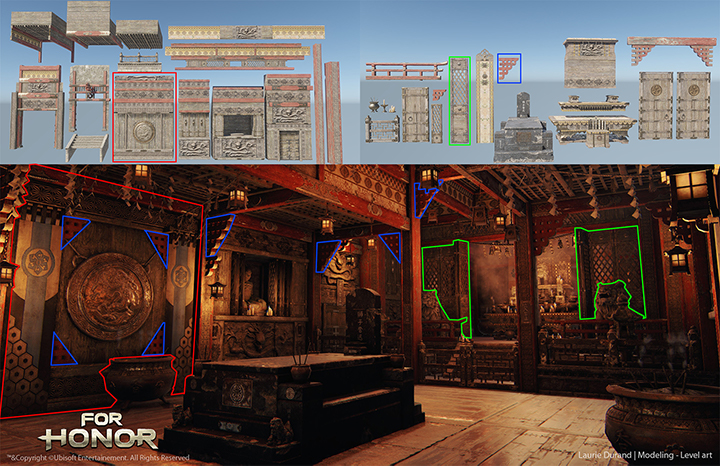
\includegraphics[width=\textwidth]{bilder/ForHonor}}
  \caption{Modulare Assets in \textit{For Honor}. In Anlehnung an \parencite{ForHonor}.}
\label{ForHonorImage}
\end{figure}
\vspace{-10.5pt}
Abbildung \ref{ForHonorImage} zeigt einen Raum, der aus einem solchen Kit entstanden ist. Ergänzend wurde er mit einigen weiteren Assets ausgestaltet. Alle Module in For Honor folgen festen Regeln, die zu Beginn der Entwicklung festgelegt wurden.  Diese Regeln umfassen die genutzte Größeneinheit, unterschiedliche Größen für verschiedene modulare Teile und das Verhalten der Assets auf dem genutzten Raster. \parencite{ForHonor}
\par
Auch viele der nicht modularen Assets in \textit{For Honor} wurden mit Hilfe der Modularität erzeugt. Der Lead Level-Designer hat zu Beginn des Projektes ein Kit aus Steinen und eines aus Holzbrettern angefertigt. Die anderen 3D-Artists konnten diese Kits nutzen, um die ihnen zugewiesenen Modelle zu erstellen. So konnten die Assets auch bei hoher Entwicklungsgeschwindigkeit mit einen großen Detailgrad entworfen werden. \parencite{ForHonor}
\par
Modularität findet mittlerweile nicht mehr nur für die Gestaltung von Levels Anwendung, sondern auch in anderen Bereichen, wie z. B. der Erstellung von Assets. Wie aufgezeigt wurde, haben sich die dafür genutzten Methoden über die letzten Jahrzehnte durchgehend geändert und verbessert. Die meisten modularen Systeme basieren allerdings immer noch auf der Nutzung von Rastern. Hauptsächlich die Methoden, wie Raster genutzt werden, haben sich weiterentwickelt. Auch aktuell werden immer neue Methoden, beispielsweise die Verwendung künstlicher Intelligenz, in die Produktionsabläufe integriert, die die Vorteile Modularität weiter ausreizen.
\newpage
\section{Modularität in der Realität}
Nicht nur in Videospielen, sondern auch in der echten Welt werden die Vorteile der Modularität ausgenutzt.
\par
Ein frühes Beispiel für Modularität ist der Gebäudebau. Eines der ersten Systeme welches den modernen Ansätzen ähnelt, wurde ca. 1830 von Henry Manning entwickelt \parencite[Abschnitt 1.1.1]{1837}. Manning verkaufte vorproduzierte Elemente, welche mit einfachen Werkzeugen zu kleinen Häusern zusammengebaut werden konnten \parencite[Abschnitt 1.1.1]{1837}.
\begin{figure}[H]
\centering
  \subfloat[][Ein Gebäude auf Basis eines Grundgerüsts \parencite{geruest}.]{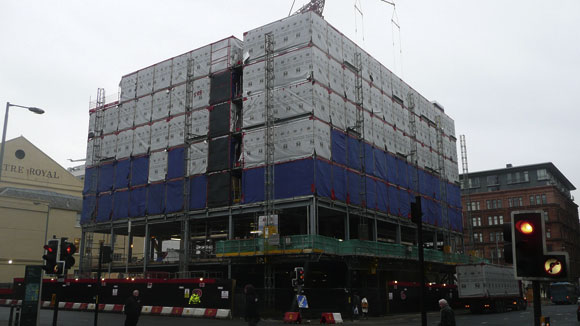
\includegraphics[height=4.3cm]{bilder/geruest}}%
  \qquad
  \subfloat[][Ein Gebäude, dessen Stabilität durch die Wände der Module entsteht \parencite{wand}.]{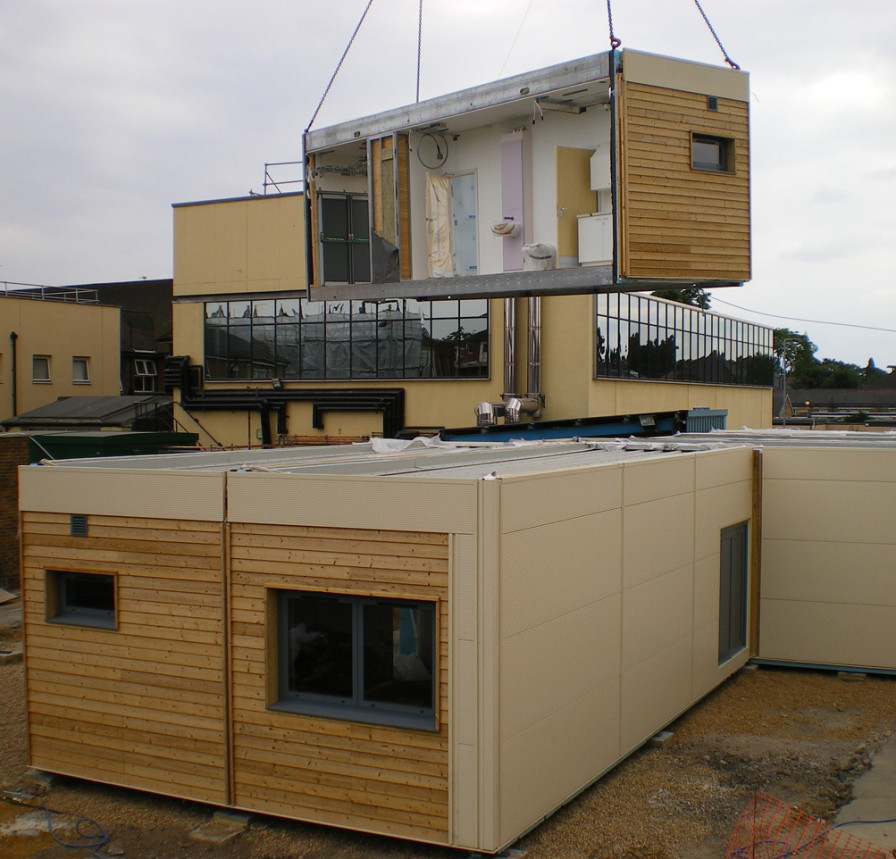
\includegraphics[height=4.3cm]{bilder/Wand}}%
  \caption{Beispiele der zwei genannten Methoden für den Bau modularer Gebäude.}%
\end{figure}
\vspace{-10.5pt}
Heutzutage werden für den Bau modularer Gebäude hauptsächlich zwei verschiedene Methoden genutzt. Erstere findet vor allem bei größeren Bauwerken Verwendung. Hier wird zuerst ein Grundgerüst gebaut, in das die Module eingesetzt werden. Die Lastverteilung verläuft hier über Eckpfeiler. Die andere Methode arbeitet mit Modulen, deren Lasten über die Wände verteilt werden. Letztere kann nur eine Höhe von 4 bis 8 Stockwerken erreichen. \parencite{Lawson}
\par
Der Produktionsablauf unterscheidet sich in vielen Punkten von der normalen Art Gebäude zu errichten, bei welcher der Großteil der Arbeit vor Ort auf der Baustelle durchgeführt wird. Die genutzten Module werden in einer Fabrik, abseits der Baustelle, angefertigt und dann vor Ort mit dem  Fundament und anderen nicht-modularen Bauelementen verbunden. So ist es (gegenüber der herkömmlichen Methode) möglich, die Bauzeit um bis zu 50\%  zu verkürzen. So können die neuen Räumlichkeiten schneller genutzt werden können und das Umfeld der Baustelle nicht so lange belastet wird, wie es normalerweise der Fall ist. \parencite{Lawson}
\par
Mit der Anzahl wiederverwendeter Module sinken die Kosten, weil das Modul nur einmal entworfen werden muss und dann immer wieder auf die gleiche Art produziert werden kann \parencite{Lawson}. Dieser Vorteil gleicht der Wiederverwendbarkeit der Module in Videospielen, die ebenfalls nur einmal designt und dann beliebig oft eingesetzt werden können.
\par
Das wohl offensichtlichste Beispiel sind LEGO-Steine. LEGO hat ein System entwickelt bei dem sich fast alle der verschiedenen produzierten Teile miteinander kombinieren lassen und das auf viele verschiedene Arten. Sechs gleichfarbige Sechser-Blöcke können auf 915.103.765 Arten \parencite[S.\,10]{LegoBuch} verbunden werden, um verschiedene Formen darzustellen. Auch die Teile der LEGO-Figuren lassen sich beliebig miteinander kombinieren. 
\par
Es existieren LEGO-Sets, die standardmäßig darauf ausgelegt sind, dass drei unterschiedliche Modelle, aus den im Set vorhandenen Teilen, gebaut werden können. Zusätzlich lassen sich, wie bei allen LEGO-Sets, noch weitere Modelle bauen, die nicht durch die Anleitung vorgegeben sind \parencite{Lego3in1}. Seit 2007 gibt es modulare Sets, die diesen Ansatz weiter verfolgen, in denen zusammengebaute kleinere Teile auf verschiedene Weisen miteinander verbunden werden können um das Aussehen des Modells auf einfache Art abzuwandeln \parencite{LegoMod}.
\begin{figure}[H]
\centering
  \makebox[\textwidth]{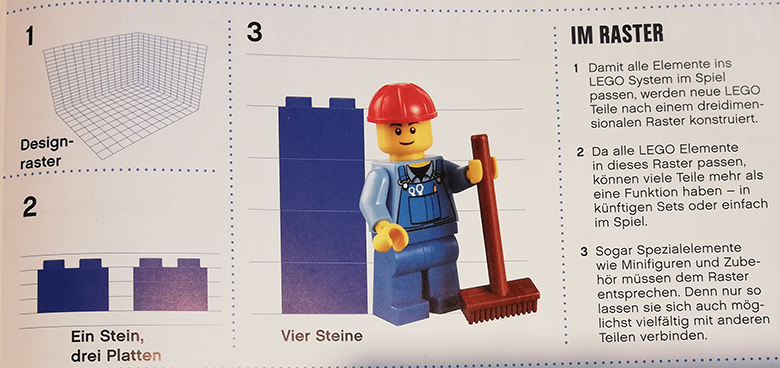
\includegraphics[width=\textwidth]{bilder/legoRaster}}
  \caption{Das Raster nach dem alle LEGO-Steine Entwickelt werden. In Anlehnung an \parencite[S.\,11]{LegoBuch}.}
\label{legoRaster}
\end{figure}
\vspace{-10.5pt}
Der modulare Ansatz ermöglicht es dem Unternehmen neue Sets zu entwerfen, die zum Beispiel den Eiffelturm darstellen, ohne dass dafür neue Teile entwickelt werden müssen. Stattdessen kann auf die bestehende Palette von LEGO-Steinen zurückgegriffen werden. Damit dies funktioniert, müssen alle Steine Regeln befolgen und auf einem bestimmten Raster entworfen werden (vgl. Abbildung \ref{legoRaster}). Hierdurch sind alle jemals entwickelten Teile zumindest stückweise miteinander kompatibel \parencite[S.\,11]{LegoBuch}.
\par
Es existieren viele weitere Anwendungsgebiete für Modularität. Die hier aufgezeigten Beispiele sollen genügen, um einen Eindruck zu vermitteln, welche Möglichkeiten und Vorteile Modularität mit sich bringen kann.
\chapter{Grundlagen der Asset-Erstellung}
In diesem Kapitel wird auf die grundlegenden Vorgehensweisen für die Erstellung und Implementierung von 3D-Modellen für Videospiele eingegangen. Da die Vorstellung aller Workflows rund um die Erstellung dreidimensionaler Modelle den Rahmen dieser Arbeit übersteigt, konzentriert sich der nachfolgende Abschnitt lediglich auf den traditionellen Ansatz.
\section{Planung}
Der erste Schritt in der Entwicklung eines Assets ist die Planung. Die Länge dieser Phase ist abhängig vom jeweiligen Projekt und dessen Fortschritt. Sind der Stil und das Setting des Spiels noch nicht definiert, wird diese Phase mehr Zeit in Anspruch nehmen.
\par
Entscheidend sind auch die Komplexität des Assets und sein geplanter Nutzen. Handelt es sich zum Beispiel um ein Fahrzeug, das der Spieler benutzen soll, müssen vorab Regeln definiert werden, die das Modell erfüllen muss, um mit der Spielfigur und der Umwelt kompatibel zu sein. Dazu gehören das Zusammenspiel mit der Spielphysik und die Beeinflussung durch die Programmierung. Für Gebäude sollte zum Beispiel die Größe der Spielfigur für Türen und Abstände in den Räumen beachtet werden. Um Problemen mit der Kamera vorzubeugen, sollte das Verhalten der Kamera bei der Planung von Decken und Wänden bedacht werden. Jedes Modell-, beziehungsweise jeder Modell-Typ, bedarf spezifischer Planung, damit es im Spiel ordnungsgemäß funktioniert. Um große Überarbeitungen in späteren Revisionen des Modells zu verhindern, sollte bereits zu Beginn sichergestellt werden, dass das geplante Modell die Regeln des Projektes einhält.
\par
Um die Umsetzung des Assets zu beschleunigen und möglichst wenig Iterationsschritte zu benötigen, sollte vor der eigentlichen Modellierungsphase ein oder mehrere Konzeptgrafiken oder wenigstens andere Referenzgrafiken vorliegen.
\newpage
\section{Modellierung}
In diesem Abschnitt werden der Aufbau eines 3D-Modells und die Arbeitsschritte in seinem Produktionsablauf erklärt. Der Abschnitt basiert im wesentlichen auf dem Handbuch von T. Beck \parencite{blender} und fasst die hier relevanten Aspekte zusammen. Bei der hier vorgestellten Methodik wird erst das Modell erzeugt und danach eine passende Textur generiert. Es ist auch möglich, diese Schritte zu vertauschen und Modelle von einer Textur ausgehend zu erzeugen. Auf dieses Verfahren wird hier aber nicht eingegangen\footnote{Der interessierte Leser findet hierfür ein Beispiel in dem \enquote{Modular Building Breakdown} von Jacob Norris \parencite{Norris}}. 
\textbf{Grundlagen und Begriffe}
\par
Grundlegend bestehen 3D-Modelle aus einer Ansammlung von Punkten in einem dreidimensionalen Raum. Diese Punkte heißen Vertex (Singular), bzw. Vertices (Plural). Eine Verbindung zwischen Zweier dieser Punkte heißt Kante oder Edge. Bilden mehrere Edges eine geschlossene Fläche, so spricht man von einem Face.
\begin{figure}[H]
\centering
  \makebox[\textwidth]{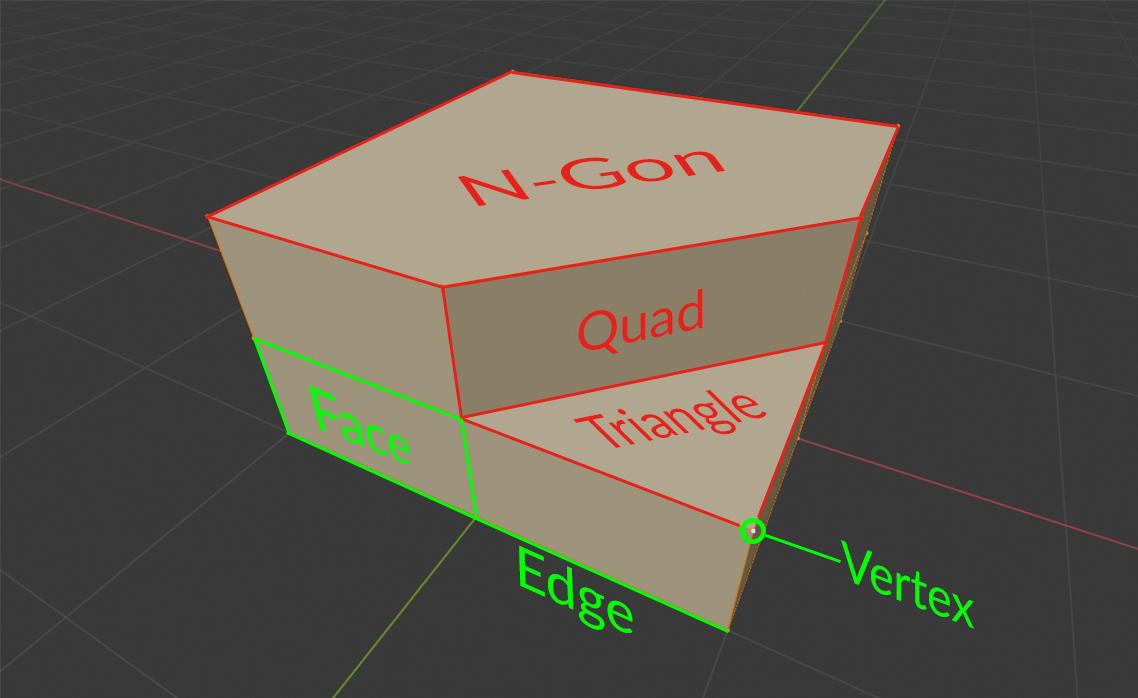
\includegraphics[width=\textwidth]{bilder/BlenderCube}}
  \caption{Darstellung der Bestandteile eines Meshes.}
\label{BlenderCube}
\end{figure}
\vspace{-10.5pt}
Wie in Abbildung \ref{BlenderCube} ersichtlich, kann die Anzahl der verwendeten Vertices zur Bildung eines Faces variieren. Man unterscheidet in der Regel zwischen Triangles (Face mit drei Vertices), Quads (Face mit vier Vertices) und N-Gons (Face mit fünf oder mehr Vertices). Im Hintergrund bestehen alle Flächen aus Dreiecken, egal, wie viele Eckpunkte sie haben \parencite[S.\,82-83]{blender}. Während des Modellierens ist es von Vorteil mit Quads zu arbeiten, sie lassen sich leichter unterteilen und wieder zu einem großen Quad zusammenführen. N-Gons sollten vermieden werden, weil diese zu Fehlern in der Darstellung und Manipulation führen können.
\par
Während Vertices und Edges die Form eines Modells definieren, repräsentieren Faces die sichtbaren Flächen des Objekts. Die Richtung, aus der eine Fläche zu sehen ist, ist abhängig von ihrer Flächennormalen. Wenn die Flächennormale nicht manipuliert wurde steht sie senkrecht auf der zugehörigen Fläche \parencite[S.88]{blender}.
\enlargethispage{10.5pt}
\newpage
Von der Flächennormalen abgewendeten Seite aus ist die Fläche unsichtbar. Es gibt in den meisten Engines eine Funktion für beidseitiges Rendern von Faces, dies ist aber sehr Performanceintensiv.
\par
Das sogenannte Shading bestimmt das Erscheinungsbild eines Meshes. Zwei spezielle Formen die direkt mit der Topologie des Models arbeiten, sind Flat und Smooth Shading.
\par
Bei der normalen Darstellung (Flat) wird jedes Face für sich gerendert, ohne die angrenzenden Faces zu beachten. Für Smooth Shading wird zwischen den Flächennormalen interpoliert, wodurch eine glattere/weichere Erscheinung des Meshes entsteht. Diese beiden Modi können auf einzelne Faces oder das gesamte Mesh angewendet werden. Dadurch sind sowohl weiche als auch harte Flächen auf einem Objekt darstellbar. \parencite[S.\,388-394]{blender}
\par
Nach den Grundlagen folgt jetzt der eigentliche Prozess der Modell-Erstellung.
\par
\textbf{Prozess der Modell-Erstellung}
\par
Für die Modell-Erstellung kommen nun die Konzeptgrafiken und Referenzen zum Einsatz. Gute Konzepte können als Blaupause im 3D-Tool genutzt werden, durch das Konzept detailgetreu nachgebildet werden kann. Auch Referenzen eignen sich, wie bereits erwähnt, um das Modell nachzubauen.
\par
Durch Manipulation der Vertices, Edges und Faces kann jede mögliche Form modelliert werden. In der Videospielproduktion wird häufig auf Low-Poly-Modelle zurückgegriffen. Das heißt, dass bei der Modellierung die Anzahl der Polygone, so gering wie möglich gehalten werden. Hierdurch verlieren die Modelle zwar an Detail, die Darstellungsgeschwindigkeit wird aber erhöht. Die fehlenden Details können teilweise im Nachhinein mit Hilfe einer Normal-Map (siehe Abschnitt \ref{Texturierung1}) ausgeglichen werden.
\par
Auch für den nächsten Arbeitsschritt hat der 3D-Artist zwei Möglichkeiten. Entweder wird zuerst das Low-Poly-Modell erstellt und aus einer Kopie dessen dann ein High-Poly-Modell, oder es wird direkt das High-Poly-Modell erstellt. Ein High-Poly-Modell ist ein Asset mit einer hohen Auflösung, in Bezug auf die genutzten Triangles. Bei letzterer Variante wird im Nachhinein durch Retopologie ein Low-Poly-Modell erzeugt.
\par
In dieser Arbeit wird der erste Ablauf zur Erstellung der 3D-Modelle genutzt.
\par
Es empfiehlt sich, die gewünschten Formen zuerst mit primitiven Objekten nachzubilden, die dann z. B. durch Unterteilen, Auftrennen, Zusammenfügen und Verformen\footnote{Dies ist nur eine Auswahl der Möglichkeiten, die zur Manipulation von Meshes zur verfügen stehen. Eine ausführliche Liste bietet das Blender Manual \parencite{blendermanual} im Kapitel Mesh Editing.} so angepasst werden können, dass das Modell den Vorgaben entspricht. Die Möglichkeiten der Mesh-Bearbeitung hängen vom genutzten 3D-Tool ab, aber alle Tools decken prinzipiell die gleichen Funktionen ab.
\newpage
In wie weit die Details der Vorgaben nachgebildet werden, hängt vom Stil, den Fähigkeiten des 3D-Artist und dem Budget\footnote{Das \enquote{Budget} bezeichnet die Menge an Ressourcen, die ein Objekt oder eine Szene verbrauchen darf, ohne dass die Performance des Spiels ungewollt beeinflusst wird.} des Models ab.
\par
Mit der Low-Poly Variante können schon erste Tests in der Engine durchgeführt werden, wie beispielsweise die Überprüfung der Vorgaben und Regeln des Projektes. Funktioniert das Modell wie geplant, kann eine Kopie, die als Basis der High-Poly-Variante dient, angelegt werden. Funktionen und Tools wie der Remesh Modifier aus Blender (vgl. Abbildung \ref{remesh}) könnem gleichmäßige Verteilungen von Flächen in Meshes erzeugt werden. Diese Gleichmäßige Verteilung ist wichtig um beim sogenannten Sculpting und auch sonstigen weiteren Anpassungen des Meshes einen konstanten Detailgrad zu erhalten \parencite{Grabstein}.
\begin{figure}[H]
\centering
  \makebox[\textwidth]{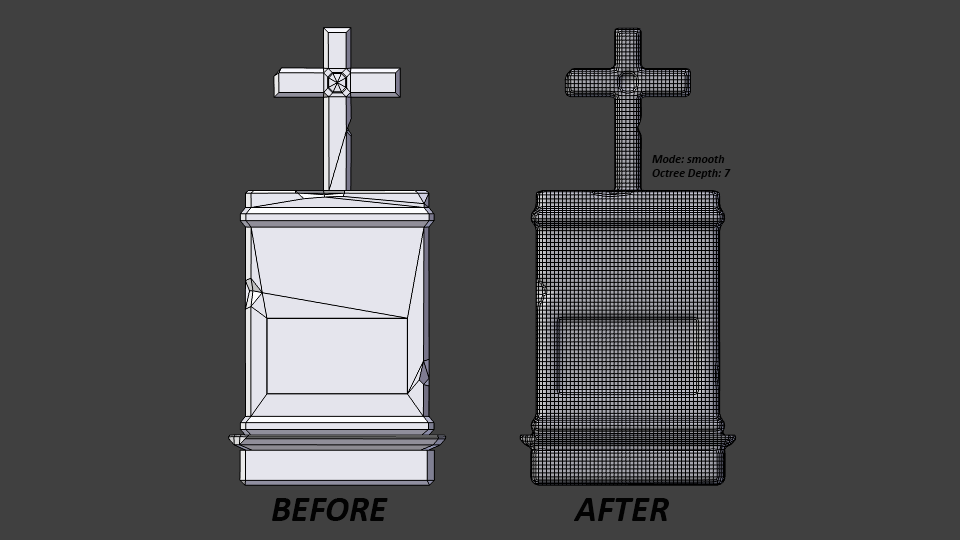
\includegraphics[width=0.7\textwidth]{bilder/remesh}}
  \caption{Ein Grabstein vor und nach dem Anwenden des Blender Remesh Modifierers \parencite{Grabstein}.}
\label{remesh}
\end{figure}
Bei der Modellierung kann mit zwei Verfahren gearbeitet werden. Entweder wird das ganze Mesh so oft unterteilt, bis es den gewünschten Detailgrad abbildet oder es wird mit dynamischer Topologie gearbeitet. Bei diesem Verfahren wird an den modifizierten Stellen neue Topologie erschaffen. So kann der Polycount des Meshes geringgehalten werden.
\par
Unabhängig von der gewählten Methode kann das Mesh anschliessend, wie Ton bearbeitet werden. Dies ermöglicht organische und detailreiche Modelle \parencite[S.\,172-189]{blender}.
\subsection{Texturierung}\label{Texturierung1}
In diesem Abschnitt wird auf Möglichkeiten eingegangen das äußere Erscheinungsbild eines Models zu verändern. Dies ist mit Hilfe von Texturen und Materialien möglich. Es werden verschiedene Arten von Texturen und ihr Einfluss auf Modelle erläutert.
\par
Die Darstellung des Models ist abhängig von dem oder den zugewiesenen Materialien. Materialien (englisch Materials) sind in allen 3D-Tools und Engines verschieden aufgebaut, funktionieren im Prinzip aber gleich. Es gibt Slots, die mit verschiedenen Texturen gefüllt werden können, und Parameter, mit denen die Erscheinung des Materials weiter beeinflusst werden kann.
\newpage
Neben den \enquote{normalen} Materialien existieren Physically Based Rendering (PBR) beziehungsweise Physically Based Shading (PBS) Materialien, der Einfachheit halber wird ab hier PBR als Überbegriff genutzt. PBR-Materialien erlauben es, annähernd physikalisch korrekte Oberflächen darzustellen. Hierfür werden Texturen mit Messwerten echter Materialien benötigt \parencite[S.\,490-492]{blender}. Dies verringert die für die Material-Erstellung benötigte Zeit, weil mögliche schrittweise Annäherung entfallen \parencite[S.\,490-492]{blender}. Des Weiteren sind PBR-Systeme in allen PBR unterstützenden 3D-Anwendungen ähnlich aufgebaut, wodurch sie unabhängig von der Anwendung gleich aussehen, ohne einer speziellen Konfiguration zu bedürfen \parencite[S.\,490-492]{blender}.  
\par
Im Folgenden werden die geläufigsten Texturen aufgelistet und ihre Funktion erklärt.\footnote{Eine Übersicht mit Beispielen und weiteren Maps ist auf dem Youtube Kanal von FlippedNormals, in dem Video Texture Maps Explained \parencite{flipped}, zu finden.} Zudem wird darauf eingegangen, ob es bei der jeweiligen Textur Unterschiede für PBR und nicht PBR gibt.
\begin{description}
	\item[Diffuse / Albedo Map]~\par
	Die Diffuse, (bzw. bei PBR-Materialien Albedo) Map, sorgt für die grundlegende Farbe des Modells. Für nicht PBR Materials sind in dieser Textur neben der Farbe auch Schattierungen und Ambient Occlusion enthalten \parencite[S.\,495]{blender}. Ambient Occlusion oder Umgebungsverdeckung erzeugt an Kanten und anderen Flächen mit geringem Abstand Verdunkelungen. Dies beruht auf dem Prinzip, dass weniger Licht an Orte gelangt, die wenig Platz für Streuung zulassen \parencite[S.\,362]{blender}. Diese Texturen können durch direktes Zeichnen auf dem Modell in einem 3D-Tool oder in einem externen Grafikprogramm angefertigt werden.
	\item[Normal Map]~\par
	Enthält ein Material Normal Maps, kann die äußere Erscheinung des Models verändert werden, ohne seine Geometrie anzupassen. So ist es möglich, Low-Poly-Modelle hochwertiger und teilweise sogar wie High-Poly-Modelle aussehen zu lassen. Die Normal Map manipuliert die Ausrichtung der Normals auf den Faces und kann so beliebige Oberflächenstrukturen vortäuschen, auch wenn das Modell eine glatte Oberfläche besitzt. Jeder Pixel der Map repräsentiert einen, über einen RGB-Wert definierten Richtungsvektor, der mit den bestehenden Normals des Models verrechnet wird. Durch diese Manipulation wird die Interaktion von Licht und Schatten mit der Oberfläche des Objektes verändert. \parencite[S.\,421-422]{blender}
	\item[Bump Map]~\par
	Bump Maps ähneln in ihrer Funktion den Normal Maps. Auch sie ändern das Erscheinungsbild des Models, ohne die Geometrie anzupassen. Der Effekt wird bei Bump Maps durch Graustufen erreicht. Schwarz stellt eine maximale Vertiefung und Weiß eine maximaler Erhöung dar, 50-prozentiges Grau lässt die Oberfläche unverändert. \parencite[S.\,420-421]{blender}
	\newpage
	\item[Displacement Map]~\par
	Das letzte Beispiel für Texturen, welche die Form der Models verändern, ist die Displacement Map. Diese verändert im Gegensatz zu den vorherigen Maps wirklich die eigentliche Geometrie des unterliegenden Objektes. Sie arbeitet wie die Bump Map mit Graustufen, Weiß führt zu einer maximalen Erhöhung und Schwarz zu einer maximalen Vertiefung, 50-prozentiges Grau steht wieder für keine Veränderung. Für eine akkurate Abbildung der Details aus der Textur benötigt das Mesh eine hohe Auflösung, folglich ist diese Methode für Spiele eher ungeeignet. Sie wird hauptsächlich für den Erstellungsprozess genutzt, um dem Modell weitere Details hinzuzufügen, die später in eine Normal Map übertragen werden. \parencite[S.\,422-423]{blender}
	\item[Specular Map]~\par
	Specular Maps werden für nicht PBR-Materialien genutzt, um zu definieren, an welchen Stellen das Modell Glanzpunkte erzeugen kann. Auch die Specular Map ist in Graustufen aufgebaut. Die Stärke des Glanzes wird durch den Grauwert bestimmt: schwarze Stellen glänzen gar nicht und weiße am stärksten. \parencite[S.\,423]{blender}
	\par
	Für PBR-Materialien werden Specular Maps nur in Sonderfällen genutzt. Eis, Wasser und Haut sind Beispiele hierfür. Die Map wird hier genutzt, um die richtige Lichtbrechung zu definieren \parencite{Jess}
	\item[Roughness / Gloss Map]~\par
	Für PBR-Materialien werden Roughness  Maps genutzt, um raue und glatte Bereiche auf einem Modell zu erzeugen. Roughness und Gloss Maps sind im Prinzip das Gleiche, aber die Auswertung des Helligkeitswerts der Textur ist invertiert. Bei einer Gloss Map repräsentiert ein heller Pixel eine sehr glatte Fläche, bei einer Roughness Map wäre die Fläche sehr rau und würde nur wenig bis keine Reflexion erzeugen. \parencite[S.\,496-497]{blender}
\end{description}
Texturen können nur auf ein Modell angewendet werden, wenn dieses entsprechend vorbereitet wurde. Dafür muss es den Prozess des UV-Unwrappings durchlaufen. Hier wird das Mesh aufgetrennt und auf eine zweidimensionale Fläche ausgebreitet. In den meisten 3D-Tools gibt es mehrere Möglichkeiten, das Mesh automatisch aufzutrennen, in der Regel ist es aber besser, diesen Vorgang manuell durchzuführen. Hierfür werden die Edges, an denen das Modell zerschnitten werden soll, markiert und im Anschluss der Unwrap-Vorgang gestartet, der das UV-Layout erzeugt. Über das UV-Layout wird definiert, welcher Ausschnitt einer Textur auf welcher Fläche des Meshes abgebildet wird. \parencite[S.\,445-455]{blender}
\par
Texturen wie die Normal Map können \enquote{gebacken} werden. Für diesen Vorgang werden eine High- und eine Low-Poly Version des gleichen Models benötigt \parencite[S.\,422]{blender}. Die Low-Poly- Version auf welche die Details des High-Poly-Meshes gebacken werden, muss unwrapped sein, damit die Details auf eine 2D-Ebene projiziert werden können \parencite[S.\,513-518]{blender}. Während des \enquote{Backens} werden die Oberflächennormalen des High-Poly-Models in die zugehörigen RGB-Werte übersetzt und in einer Normal Map gespeichert \parencite[S.\,422]{blender}.
\enlargethispage{10.5pt}
\par
Für Spiele wie zum Beispiel \textit{World of Warcraft} (Blizzard Entertainment, 2004) werden nur Low-Poly- Modelle mit Diffuse Texturen genutzt, die nur die Farbe des Modells enthalten \parencite{WoW}. Für die Erstellung dieser Texturen werden High-Poly-Meshes genutzt, deren Details dann auf verschiedene Texturen gebacken werden und anschließend in einer Diffuse Map zusammen geführt werden \parencite{WoW}. Mit dieser Methode wird ein spezieller Look erzeugt und die Speichernutzung wird reduziert.
\par
Mit den sogenannten 3D-Zeichenprogrammen, wie beispielsweise Substance Painter, können Materialien mit allen benötigten Texturen auf 3D Modelle angewendet werden. So können bestehende Materialien manipuliert oder neue angelegt werden. Die Materialien können auf die Beschaffenheiten des Modells eingehen und zum Beispiel Verschleiß an Kanten simulieren. So können in kurzer Zeit detailreiche, realistische Materialien erzeugt werden.
\par
Alle Materialien müssen vor dem Export aus dem 3D-Tool allen zugehörigen Faces des Objekts zugewiesen sein und die Quads des Models sollten in Triangles übersetzt werden (\enquote{Triangulation}). Game-Engines arbeiten nur mit Triangles und übersetzen das Modell selber in Triangles wenn es aus Quads und N-Gons besteht. Bei diesem Vorgang kann es zu Fehlern mit den Normalen kommen. Wird die Triangulation vor dem Export durchgeführt, sind diese Fehler vermeidbar.
\section{Implementierung}\label{Implementierung1}
Für die Erstellung eines Videospiels mit den angefertigten Assets wird eine Game-Engine benötigt. Alle in der Engine verwendeten Modelle werden in einen Verbund aus Dreiecken übersetzt, weil Grafikkarten (GPUs) mit Dreiecken rechnen \parencite{gpu}. Jedes Mesh wird in der Game Engine in zwei Teilen abgespeichert, dem Vertex Buffer und dem Index Buffer \parencite{gpu}. Der Vertex Buffer enthält eine Liste aller Vertices des Meshes \parencite{gpu}. Dazu gehören Position des Vertex, UV-Koordinaten, Ausrichtung der Normals und weitere \parencite{gpu}. Der Index Buffer enthält Informationen darüber, welche Vertices miteinander Dreiecke bilden und so das Mesh formen \parencite{gpu}. Zusätzlich zu dem Index und Vertex Buffer werden dem Mesh ein oder mehrere Materialien zugewiesen \parencite{gpu}. 
\par
Die Materialien werden in der Engine selbst erstellt und mit den vorgesehenen Texturen konfiguriert. Sie können nicht aus 3D-Tools, mit denen das Mesh erstellt wurde, übernommen werden. Die Material-Systeme der Engines und die der 3D-Tools sind nicht kompatibel.
\newpage
Für die Darstellung des Meshes auf dem Bildschirm wird für jeden Frame eine Folge von Schritten durchlaufen, die sich wie folgt zusammenfassen lassen:
\begin{enumerate}
\item Im ersten Schritt, dem \textit{Input Assembly}, werden anhand des Index Buffers die Vertices aus dem Vertex Buffer miteinander zu Dreiecken verbunden.
\item Dann findet das \textit{Vertex Shading} statt, bei dem die aktuelle Ausrichtung und Position des Meshes in Relation zur Kamera mit allen Vertices verrechnet wird. So wird die Gesamtansicht bestimmt und welche Teile des Objektes zu sehen sind.
\item Die \textit{Rasterization} erzeugt aus jedem Triangle eine gerasterte Fläche, über die die Vertex-Normalen, UV-Koordinaten und weitere Eigenschaften der Vertices interpoliert werden.
\item Der Schritt des \textit{Pixel Shading} ordnet jedem Pixel in der gerasterten Fläche abhängig von Material, Licht und anderen Einflüssen eine Farbe zu.
\item  Zuletzt wird \textit{Render Target Output} durchgeführt, um die berechneten Werte für die Darstellung weiterzuleiten. Es gibt einen Zwischenschritt, der überprüft, ob die errechneten Pixel angezeigt werden sollen. Es wird unter anderem überprüft, ob Pixel nicht sichtbar sind, weil das zugehörige Objekt von einem anderen Objekt verdeckt wird oder ob ein Pixel durchsichtig ist. Dann wird der dahinterliegende Pixel genutzt.
\vspace{-10.5pt}
\begin{flushright}\parencite{gpu}\end{flushright}
\end{enumerate}
Das Rendering ist damit abgeschlossen.
\par
Die Grafikkarte wird bei der Bearbeitung von Bildern von der CPU unterstützt. Diese sendet Draw Calls an die Grafikkarte und übergibt der Grafikkarte die benötigten Daten, um den Draw Call auszuführen. Ein Draw Call enthält Information über das zu rendernde Mesh, sein Material und seine sonstigen Eigenschaften. Jeder Draw Call wird vom Grafikkarten-Treiber übersetzt und auf Fehler überprüft. Dadurch entstehen für jeden Draw Call Grundkosten, die sich in verbrauchter Zeit widerspiegeln. Für jedes Material wird ein eigener Draw Call abgesetzt; das heißt, wenn ein Mesh mit drei Materials ausgestattet ist, löst es auch drei Draw Calls aus.
\par
Weil die Grafikkarte von der CPU abhängig ist und die CPU jeden Draw Call durcharbeiten muss, haben diese einen direkten Einfluss auf die Framerate. Die Anzahl an Draw Calls sollte folglich gering gehalten werden. \parencite{gpu}
\par
In der Engine kann der Aufbau eines Objektes nicht geändert werden, lediglich Skalierung und Rotation können angepasst werden. Das hat aber keinen Einfluss auf die Struktur der Vertices, Faces und Edges. Objekte können für leichtere Handhabung und das Verringern von Draw Calls mit einander verknüpft werden. Dies hat keinen Einfluss auf die Struktur der verbundenen Objekte.
\par
Moderne Spiele können nur die, von der Spielerkamera erfassten, Objekte rendern. Dieser Prozess nennt sich auch Occlusion Culling. Deshalb sollten Objekte nicht unbegrenzt verbunden werden.  Ist nur ein kleiner Teil des Objektes zu sehen, wird dieses komplett gerendert und sorgt so für einen weiteren kompletten Draw Call, wodurch gegebenenfalls Performance verschwendet wird. Ob ein Objekt zu sehen ist, wird am Anfang des Prozesses mit einer Bounding Box überprüft\footnote{Eine Bounding Box ist ein Quader um die maximalen Maße des Objektes.}. Es kann dann passieren, dass zwar die Bounding Box gesehen wird, das Objekt an sich aber nicht. So würden wieder unnötige Draw Calls gestartet werden. \parencite{gpu}
\par
Eine Möglichkeit Draw Calls weiter zu verringern, ist das wiederholte Benutzen des gleichen Objektes mit \textit{Instancing}. Aktuelle Engines erkennen dies automatisch. Es wird dann nur ein Draw Call abgesetzt, der die verschiedenen Konfigurationen, Position, Rotation etc. der einzelnen Objekte beinhaltet. \parencite{gpu}
\par
Durch das Verbinden von Texturen zu einer größeren Textur, einem so genannten Textur Atlas, können die Draw Calls weiter reduziert werden. Mit Textur-Atlanten können mit einem Material verschiedene Oberflächen dargestellt werden. So können mehrere Objekte mit dem gleichen Material ausgestattet werden, für das aber nur ein Draw Call erzeugt wird. \parencite{gpu} 
\par
Die Grundlagen der Asset-Erstellung und -Implementierung sind hiermit abgeschlossen. Das folgende Kapitel behandelt Methoden, zur Erstellung und Verwendung modularer Assets. Des Weiteren wird auf deren Anforderungen und mögliche Vor- und Nachteile eingegangen. 